\documentclass[../main.tex]{subfiles}

\graphicspath{{../images/}}

\begin{document}
\pagestyle{fancy}
\lhead{Junseo Shin \& Jeremy Smith}
\rhead{Lab Notebook: Fourier Methods}
\chead{9/17/24-9/19/24}
\section{The Fluxgate Magetometer}

% chapter 13
\subsection*{Chapter 13: Understanding the Fluxgate Magnetometer}
\addcontentsline{toc}{subsection}{Chapter 13: Understanding the Fluxgate Magnetometer}
\paragraph{Notes}

\begin{itemize}
    \item Teachspin Fluxgate Magnetometer Module:
    \begin{itemize}
        \item Fluxgate Sensor: 
        \item Double Solenoid: Two electrically separate wires are wound and stored in a tube for the fluxgate sensor to fit in. This is so we can have up to two independently added magnetic fields. 
        \begin{itemize}
            \item Solenoid pitch $= 2.54$ mm, and the expected magnetic field inside the Solenoid is given by
           \begin{align*}
               B_\text{ext} = 2 \mu_0 n i
           \end{align*} 
            where $i$ is the current through a solenoid, $2$ accounts for the doubled layer, and the turn density is
            \begin{align*}
                n = 1 \textrm{ turn} / (\qty{0.00254}{m} = \qty{394}{m^{-1}} 
            \end{align*}
            From this, the magnitude of the external magnetic field given a current $i$ is
            \begin{align*}
                \frac{B_\text{ext}}{i} = 2 \cdot (4 \pi \qty{e-7}{T m / A}) \qty{394}{/m} = \qty{990}{\micro T/A}
            \end{align*}
        \end{itemize}
        \item Modeling Output: Calibrating the Solenoid
        \begin{itemize}
            \item For simple models the 2$f$-component of the field is linear $A = S B_\text{ext}$, but we are actually measuring the magnitude of the spectral component
            \begin{align*}
                M = S \abs{B_\text{ext}}
            \end{align*}
            \item The geometry of the vector components require us to take a phaser sum which gives us the square magnitude of the measured field
            \begin{align*}
                M^s = S^2 \qt[
                    \qt(
                        B_\text{ext} + \frac{A_{para}}{S}
                    )^2 + \qt(
                        \frac{A_{perp}}{S}
                    )^2
                    )
                ] = S^2 \qt[(B_{ext} + a)^2 + b^2]
            \end{align*}
        \end{itemize}
    \end{itemize}
 
\end{itemize}

% fig exp3_1.png and exp3_2.png
\begin{figure}[ht]
    \centering
    \begin{tabular}{cc}
        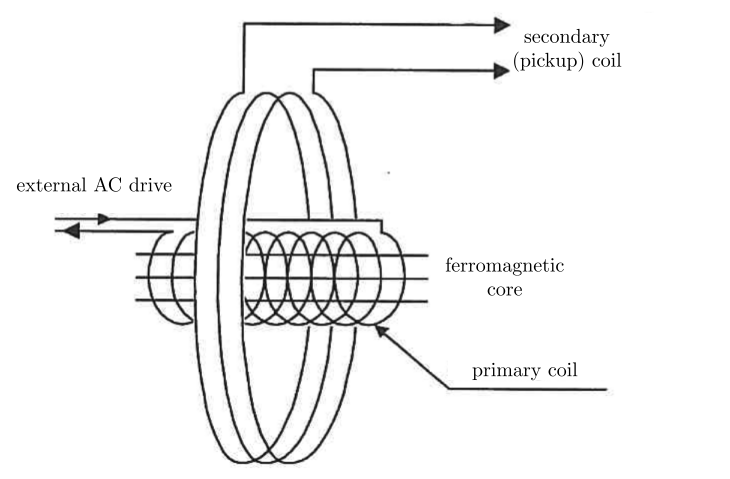
\includegraphics[width=0.45\linewidth]{exp3_1.png} & 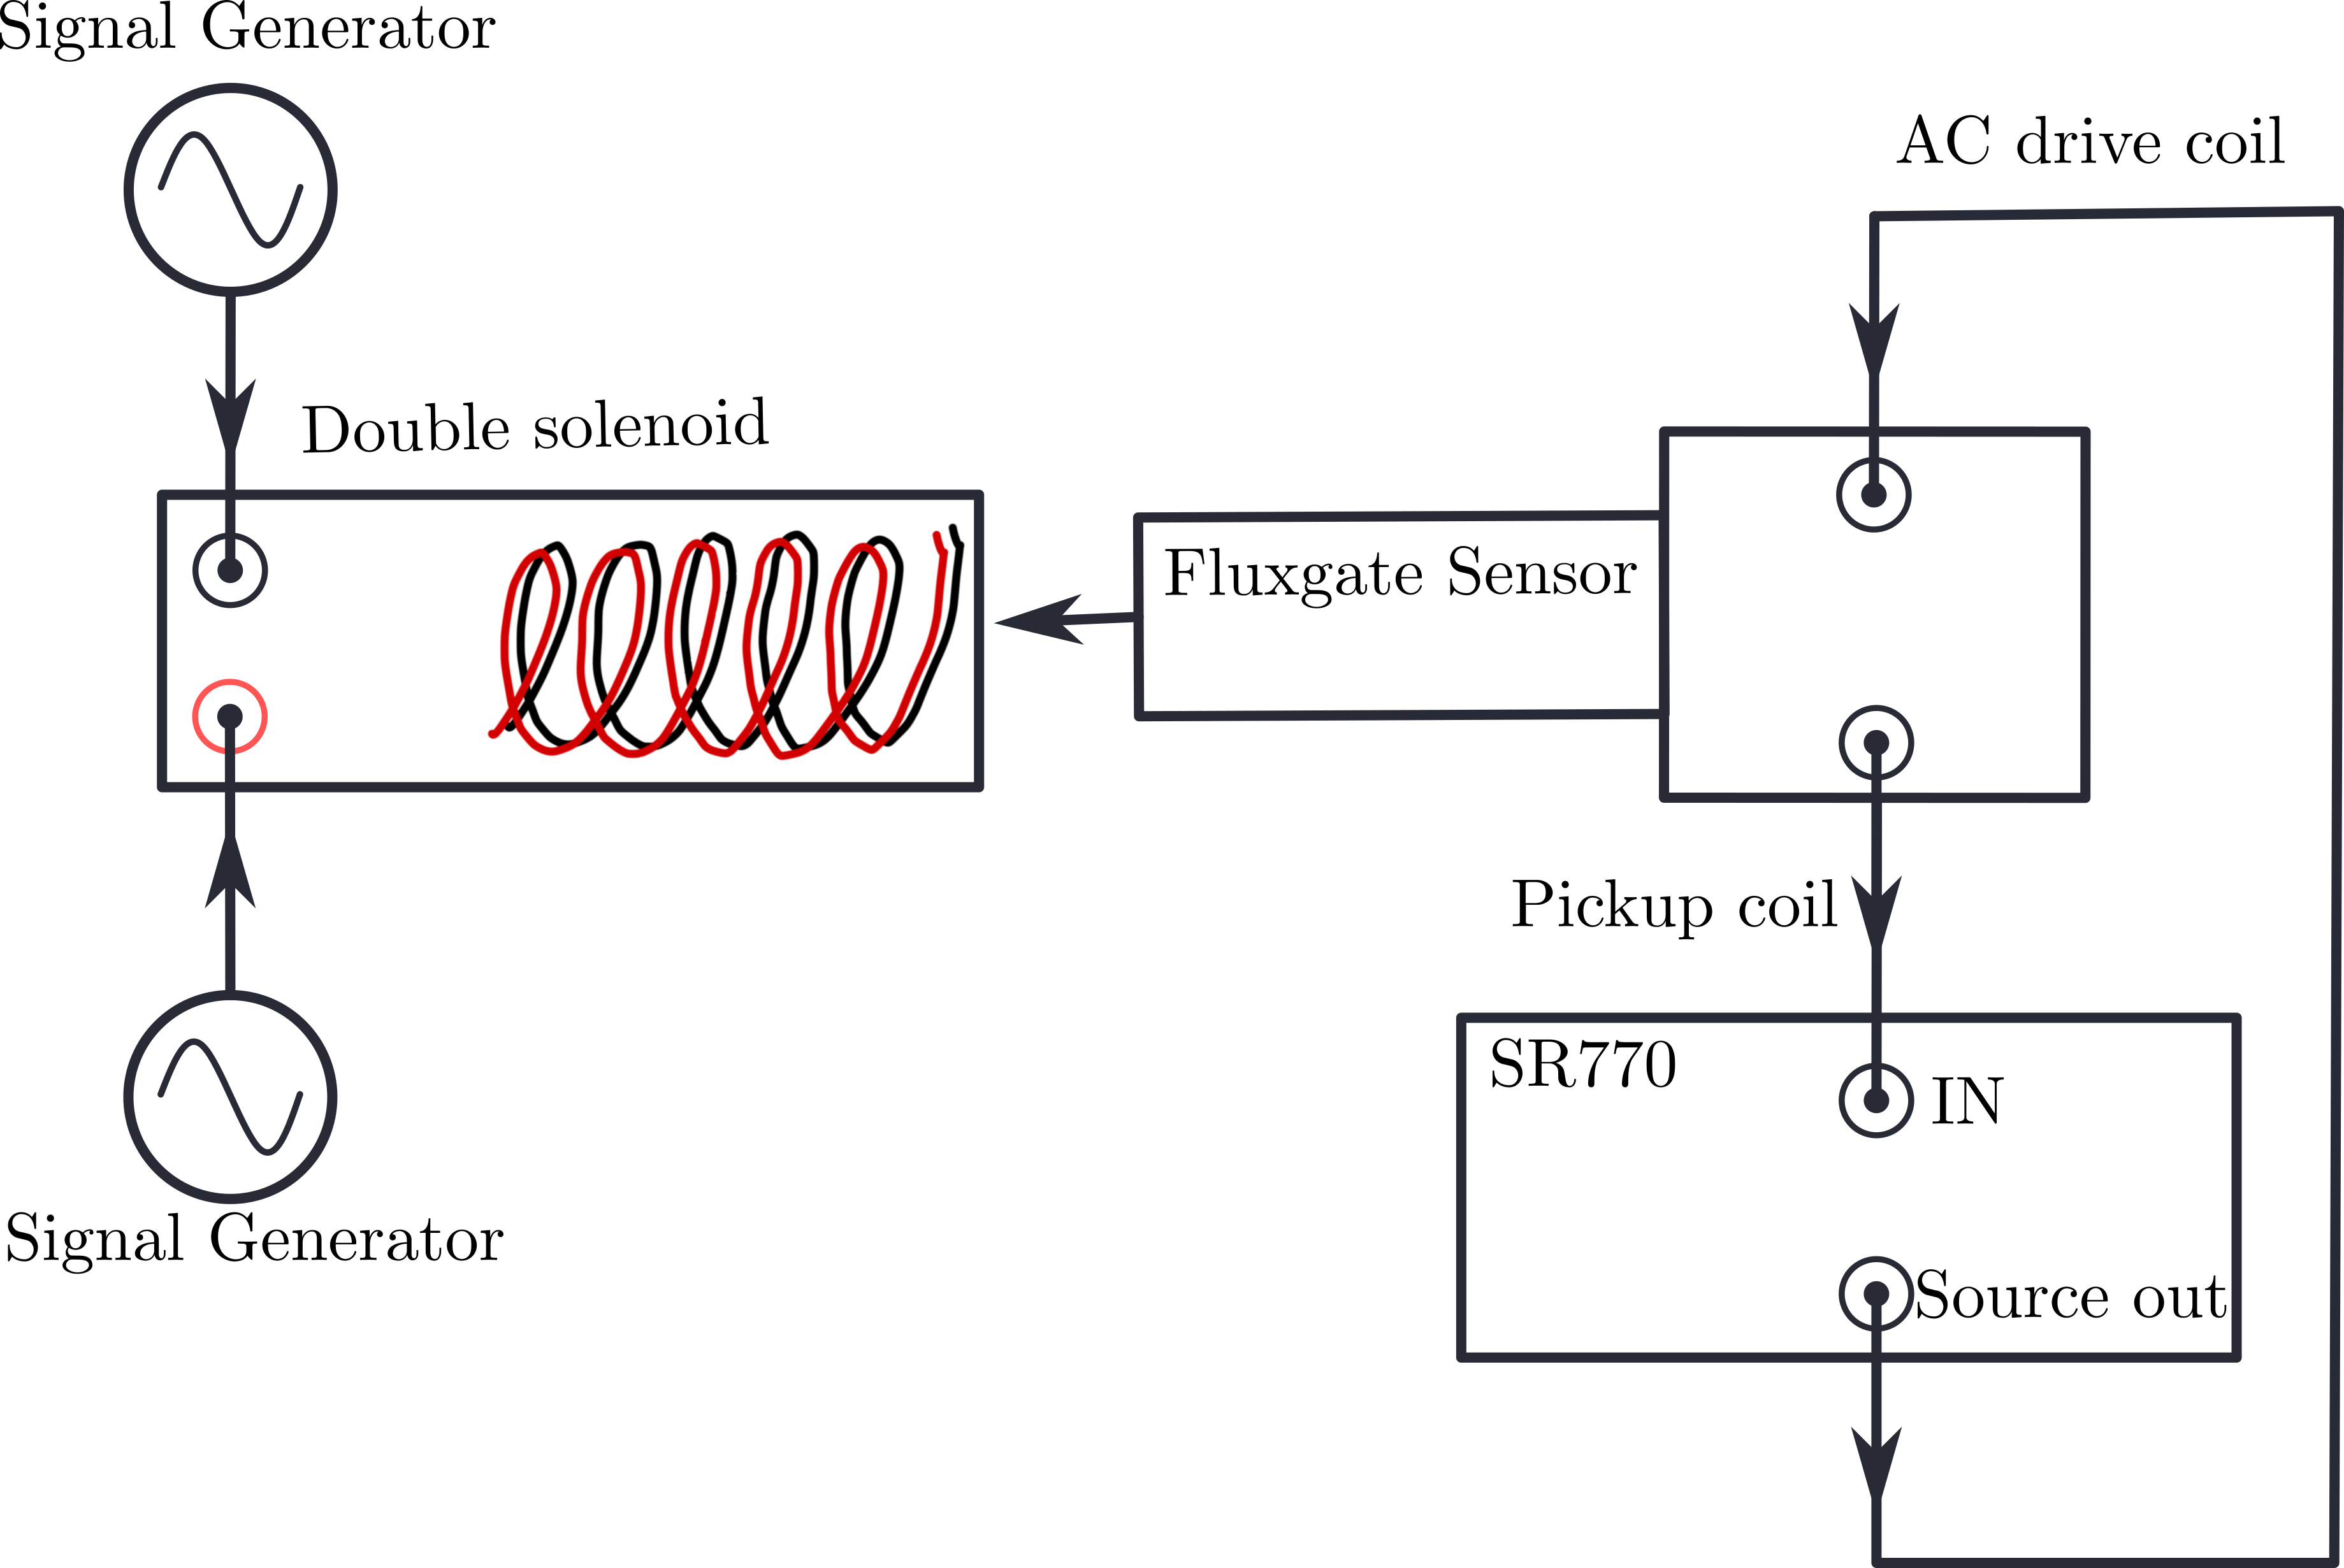
\includegraphics[width=0.45\linewidth]{exp3_2.png} \\
        (a) Fluxgate Magnetometer sensor components & (b) Fluxgate sensor and double solenoid setup \\
    \end{tabular}
    \caption{(a) Fluxgate Magnetometer sensor components and (b) Fluxgate sensor and double solenoid setup}
    \label{fig:exp3_combined}
\end{figure}

\paragraph{Experimental Setup}
\begin{itemize}
    \item SR770 Config:
    \begin{itemize}
        \item FREQ: SPAN 3.125 kHz for observation, 12.2 Hz for measurement; Center Freq. 2 kHZ (second harmonic)
        \item MEASure: PSD, Flattop Window
        \item Average: 16, Exponential
        \item SOURCE OUT: 1 kHz 1 V 
    \end{itemize}
\end{itemize}

\paragraph{Procedure}
\begin{itemize}
    \item 770: 1 kHz 1 V Sine SOURCE OUT $\to$ Power Audio Amp. module and adjust gain to 6 V (monitor output with splitter to scope)
    \item Power Audio Amp. output $\to$ Fluxgate Primary (AC drive) coil
    \item Secondary (pick-up) coil $\to$ SR770 input
    \item Place the Fluxgate sensor in the double solenoid pointing straight down   
    \item Measure second harmonic $2f$ component of the frequency spectrum
    \item Add 2.5 V DC current (from 33500 B) to Solenoid A and measure the changes in the $2f$ component
    \begin{itemize}
        \item NOTE: Use 50 Ohm Terminator so the measured ouput voltage is exactly the displayed voltage due to the internal 50 Ohm impedence of the 33500B
    \end{itemize}
    \item 770 config change: FREQ SPAN 12.2 Hz
    \item Solenoid A: Replace DC current with AC ($f_A = 5$ Hz 1 V Sine wave from 33500B) and find the $2f \pm f_A$ components
    \item Solenoid B: Add a second AC drive ($f_B = 2.5$ Hz 0.5 V Sine wave from second 33500 B) and measure the four side band frequencies $2f \pm f_A, 2f \pm f_B$
\end{itemize}

\paragraph{Observations}

\end{document}